%! Author = Omar Iskandarani
%! Title = From Quantum Constants to Galactic Swirl: Deriving Æther Density in the VAM Framework
%! Date = June 17, 2025
%! Affiliation = Independent Researcher, Groningen, The Netherlands
%! License = © 2025 Omar Iskandarani. All rights reserved. This manuscript is made available for academic reading and citation only. No republication, redistribution, or derivative works are permitted without explicit written permission from the author. Contact: info@omariskandarani.com
%! ORCID = 0009-0006-1686-3961
%! DOI = 10.5281/zenodo.15750583

% === Metadata ===
\newcommand{\papertitle}{\textbf{From Quantum Constants to Galactic Swirl: Deriving Æther Density in the VAM Framework}}
\newcommand{\paperdoi}{10.5281/zenodo.15750583}


\documentclass[12pt]{article}
\usepackage{amssymb}
% vamstyle.sty
\NeedsTeXFormat{LaTeX2e}
\ProvidesPackage{vamstyle}[2025/07/01 VAM unified style]

% === Constants ===
\newcommand{\hbarVal}{\ensuremath{1.054571817 \times 10^{-34}}} % J\cdot s
\newcommand{\meVal}{\ensuremath{9.10938356 \times 10^{-31}}} % kg
\newcommand{\cVal}{\ensuremath{2.99792458 \times 10^{8}}} % m/s
\newcommand{\alphaVal}{\ensuremath{1 / 137.035999084}} % unitless
\newcommand{\alphaGVal}{\ensuremath{1.75180000 \times 10^{-45}}} % unitless
\newcommand{\reVal}{\ensuremath{2.8179403227 \times 10^{-15}}} % m
\newcommand{\rcVal}{\ensuremath{1.40897017 \times 10^{-15}}} % m
\newcommand{\vacrho}{\ensuremath{5 \times 10^{-9}}} % kg/m^3
\newcommand{\LpVal}{\ensuremath{1.61625500 \times 10^{-35}}} % m
\newcommand{\MpVal}{\ensuremath{2.17643400 \times 10^{-8}}} % kg
\newcommand{\tpVal}{\ensuremath{5.39124700 \times 10^{-44}}} % s
\newcommand{\TpVal}{\ensuremath{1.41678400 \times 10^{32}}} % K
\newcommand{\qpVal}{\ensuremath{1.87554596 \times 10^{-18}}} % C
\newcommand{\EpVal}{\ensuremath{1.95600000 \times 10^{9}}} % J
\newcommand{\eVal}{\ensuremath{1.60217663 \times 10^{-19}}} % C

% === VAM/\ae ther Specific ===
\newcommand{\CeVal}{\ensuremath{1.09384563 \times 10^{6}}} % m/s
\newcommand{\FmaxVal}{\ensuremath{29.0535070}} % N
\newcommand{\FmaxGRVal}{\ensuremath{3.02563891 \times 10^{43}}} % N
\newcommand{\gammaVal}{\ensuremath{0.005901}} % unitless
\newcommand{\GVal}{\ensuremath{6.67430000 \times 10^{-11}}} % m^3/kg/s^2
\newcommand{\hVal}{\ensuremath{6.62607015 \times 10^{-34}}} % J Hz^-1

% === Electromagnetic ===
\newcommand{\muZeroVal}{\ensuremath{1.25663706 \times 10^{-6}}}
\newcommand{\epsilonZeroVal}{\ensuremath{8.85418782 \times 10^{-12}}}
\newcommand{\ZzeroVal}{\ensuremath{3.76730313 \times 10^{2}}}

% === Atomic & Thermodynamic ===
\newcommand{\RinfVal}{\ensuremath{1.09737316 \times 10^{7}}}
\newcommand{\aZeroVal}{\ensuremath{5.29177211 \times 10^{-11}}}
\newcommand{\MeVal}{\ensuremath{9.10938370 \times 10^{-31}}}
\newcommand{\MprotonVal}{\ensuremath{1.67262192 \times 10^{-27}}}
\newcommand{\MneutronVal}{\ensuremath{1.67492750 \times 10^{-27}}}
\newcommand{\kBVal}{\ensuremath{1.38064900 \times 10^{-23}}}
\newcommand{\RVal}{\ensuremath{8.31446262}}

% === Compton, Quantum, Radiation ===
\newcommand{\fCVal}{\ensuremath{1.23558996 \times 10^{20}}}
\newcommand{\OmegaCVal}{\ensuremath{7.76344071 \times 10^{20}}}
\newcommand{\lambdaCVal}{\ensuremath{2.42631024 \times 10^{-12}}}
\newcommand{\PhiZeroVal}{\ensuremath{2.06783385 \times 10^{-15}}}
\newcommand{\phiVal}{\ensuremath{1.61803399}}
\newcommand{\eVVal}{\ensuremath{1.60217663 \times 10^{-19}}}
\newcommand{\GFVal}{\ensuremath{1.16637870 \times 10^{-5}}}
\newcommand{\lambdaProtonVal}{\ensuremath{1.32140986 \times 10^{-15}}}
\newcommand{\ERinfVal}{\ensuremath{2.17987236 \times 10^{-18}}}
\newcommand{\fRinfVal}{\ensuremath{3.28984196 \times 10^{15}}}
\newcommand{\sigmaSBVal}{\ensuremath{5.67037442 \times 10^{-8}}}
\newcommand{\WienVal}{\ensuremath{2.89777196 \times 10^{-3}}}
\newcommand{\kEVal}{\ensuremath{8.98755179 \times 10^{9}}}

% === \ae ther Densities ===
\newcommand{\rhoMass}{\rho_\text{\ae}^{(\text{mass})}}
\newcommand{\rhoMassVal}{\ensuremath{3.89343583 \times 10^{18}}}
\newcommand{\rhoEnergy}{\rho_\text{\ae}^{(\text{energy})}}
\newcommand{\rhoEnergyVal}{\ensuremath{3.49924562 \times 10^{35}}}
\newcommand{\rhoFluid}{\rho_\text{\ae}^{(\text{fluid})}}
\newcommand{\rhoFluidVal}{\ensuremath{7.00000000 \times 10^{-7}}}

% === Draft Options ===
\newif\ifvamdraft
% \vamdrafttrue
\ifvamdraft
\RequirePackage{showframe}
\fi

% === Load Once ===
\RequirePackage{ifthen}
\newboolean{vamstyleloaded}
\ifthenelse{\boolean{vamstyleloaded}}{}{\setboolean{vamstyleloaded}{true}

% === Page ===
\RequirePackage[a4paper, margin=2.5cm]{geometry}

% === Fonts ===
\RequirePackage[T1]{fontenc}
\RequirePackage[utf8]{inputenc}
\RequirePackage[english]{babel}
\RequirePackage{textgreek}
\RequirePackage{mathpazo}
\RequirePackage[scaled=0.95]{inconsolata}
\RequirePackage{helvet}

% === Math ===
\RequirePackage{amsmath, amssymb, mathrsfs, physics}
\RequirePackage{siunitx}
\sisetup{per-mode=symbol}

% === Tables ===
\RequirePackage{graphicx, float, booktabs}
\RequirePackage{array, tabularx, multirow, makecell}
\newcolumntype{Y}{>{\centering\arraybackslash}X}
\newenvironment{tighttable}[1][]{\begin{table}[H]\centering\renewcommand{\arraystretch}{1.3}\begin{tabularx}{\textwidth}{#1}}{\end{tabularx}\end{table}}
\RequirePackage{etoolbox}
\newcommand{\fitbox}[2][\linewidth]{\makebox[#1]{\resizebox{#1}{!}{#2}}}

% === Graphics ===
\RequirePackage{tikz}
\usetikzlibrary{3d, calc, arrows.meta, positioning}
\RequirePackage{pgfplots}
\pgfplotsset{compat=1.18}
\RequirePackage{xcolor}

% === Code ===
\RequirePackage{listings}
\lstset{basicstyle=\ttfamily\footnotesize, breaklines=true}

% === Theorems ===
\newtheorem{theorem}{Theorem}[section]
\newtheorem{lemma}[theorem]{Lemma}

% === TOC ===
\RequirePackage{tocloft}
\setcounter{tocdepth}{2}
\renewcommand{\cftsecfont}{\bfseries}
\renewcommand{\cftsubsecfont}{\itshape}
\renewcommand{\cftsecleader}{\cftdotfill{.}}
\renewcommand{\contentsname}{\centering \Huge\textbf{Contents}}

% === Sections ===
\RequirePackage{sectsty}
\sectionfont{\Large\bfseries\sffamily}
\subsectionfont{\large\bfseries\sffamily}

% === Bibliography ===
\RequirePackage[numbers]{natbib}

% === Links ===
\RequirePackage{hyperref}
\hypersetup{
    colorlinks=true,
    linkcolor=blue,
    citecolor=blue,
    urlcolor=blue,
    pdftitle={The Vortex \AE ther Model},
    pdfauthor={Omar Iskandarani},
    pdfkeywords={vorticity, gravity, \ae ther, fluid dynamics, time dilation, VAM}
}
\urlstyle{same}
\RequirePackage{bookmark}

% === Misc ===
\RequirePackage[none]{hyphenat}
\sloppy
\RequirePackage{empheq}
\RequirePackage[most]{tcolorbox}
\newtcolorbox{eqbox}{colback=blue!5!white, colframe=blue!75!black, boxrule=0.6pt, arc=4pt, left=6pt, right=6pt, top=4pt, bottom=4pt}
\RequirePackage{titling}
\RequirePackage{amsfonts}
\RequirePackage{titlesec}
\RequirePackage{enumitem}

\AtBeginDocument{\RenewCommandCopy\qty\SI}

\pretitle{\begin{center}\LARGE\bfseries}
\posttitle{\par\end{center}\vskip 0.5em}
\preauthor{\begin{center}\large}
\postauthor{\end{center}}
\predate{\begin{center}\small}
\postdate{\end{center}}

\endinput
}
% vamappendixsetup.sty

\newcommand{\titlepageOpen}{
  \begin{titlepage}
  \thispagestyle{empty}
  \centering
  {\Huge\bfseries \papertitle \par}
  \vspace{1cm}
  {\Large\itshape\textbf{Omar Iskandarani}\textsuperscript{\textbf{*}} \par}
  \vspace{0.5cm}
  {\large \today \par}
  \vspace{0.5cm}
}

% here comes abstract
\newcommand{\titlepageClose}{
  \vfill
  \null
  \begin{picture}(0,0)
  % Adjust position: (x,y) = (left, bottom)
  \put(-200,-40){  % Shift 75pt left, 40pt down
    \begin{minipage}[b]{0.7\textwidth}
    \footnotesize % One step bigger than \tiny
    \renewcommand{\arraystretch}{1.0}
    \noindent\rule{\textwidth}{0.4pt} \\[0.5em]  % ← horizontal line
    \textsuperscript{\textbf{*}}Independent Researcher, Groningen, The Netherlands \\
    Email: \texttt{info@omariskandarani.com} \\
    ORCID: \texttt{\href{https://orcid.org/0009-0006-1686-3961}{0009-0006-1686-3961}} \\
    DOI: \href{https://doi.org/\paperdoi}{\paperdoi} \\
    License: CC-BY 4.0 International \\
    \end{minipage}
  }
  \end{picture}
  \end{titlepage}
}
\begin{document}

    % === Title page ===
    \titlepageOpen

    \begin{abstract}
        This paper presents a first-principles derivation of the æther density within the Vortex \AE{}ther Model (VAM)—a topological fluid-dynamic framework in which gravity, inertia, and quantum behavior emerge from structured vorticity in an inviscid, compressible medium. We derive the æther’s mass density \( \rho_{\text{\ae}}^{\text{(fluid)}} \) and rotational energy density \( \rho_{\text{\ae}}^{\text{(energy)}} \) without circular dependence on empirical gravitational constants.

        By anchoring the characteristic vorticity \( \vec{\omega} \) to the electron’s Compton frequency, scaled by the fine-structure constant \( \alpha \), and evaluating the swirl energy over a volume defined by the classical electron radius \( r_e \), we obtain:
        \[
            \rho_{\text{\ae}}^{\text{(fluid)}} = \frac{2 m_e c^2}{\left( \alpha \cdot \frac{m_e c^2}{\hbar} \right)^2 \cdot \left( r_e^3 / 3 \right)} \approx 7 \times 10^{-7} \, \text{kg/m}^3
        \]
        This value matches vacuum energy estimates and vorticity energy densities from both cosmology and quantum fluid analogs.

        We further construct a two-component swirl velocity profile—combining a finite-core vortex solution with a saturating ætheric tail—which yields a closed-form expression for galactic rotation curves without invoking dark matter or MOND interpolation. The resulting profile predicts long-range vorticity-induced acceleration, ætheric pressure gradients, swirl-based time dilation, and quantized circulation surfaces. This formulation bridges microscopic and galactic scales through shared physical parameters and offers direct falsifiability in both astrophysical and subatomic regimes.
    \end{abstract}


    \titlepageClose

% ============= Begin of content ============




    \section{Introduction}

    In VAM~\cite{iskandarani2025vam2}, the \AE{}ther is a structured, inviscid medium supporting vorticity and energy transfer. Two key densities are defined:
    \begin{itemize}
        \item $\rho_{\text{\ae}}^{\text{(fluid)}}$: mass density akin to a classical fluid.
        \item $\rho_{\text{\ae}}^{\text{(energy)}}$: energy density stored in vorticity.
    \end{itemize}

    \begin{table}[H]
        \footnotesize
        \centering
        \renewcommand{\arraystretch}{1.2}
        \begin{tabular}{|l|p{10.5cm}|}
            \hline
            \textbf{Prediction} & \textbf{Description} \\
            \hline
            \(\rho_{\text{\ae}}^{\text{(fluid)}}\) & Derived æther fluid density matches quantum and cosmological estimates: \( \sim 7 \times 10^{-7} \, \text{kg/m}^3 \). \\
            \hline
            \(\rho_{\text{\ae}}^{\text{(energy)}}\) & Core vorticity energy density reaches \( \sim 8.4 \times 10^{35} \, \text{J/m}^3 \), consistent with Planck-scale tension. \\
            \hline
            Galaxy Rotation Curves & Combined vortex + swirl tail velocity law reproduces flat galaxy rotation curves without dark matter. \\
            \hline
            Residual Acceleration & Predicts background swirl-induced acceleration \( a_{\text{swirl}} = r \omega_{\text{bg}}^2 \), with \( \omega_{\text{bg}} \approx 0.12 \, \text{s}^{-1} \). \\
            \hline
            Refractive Index Shift & Predicts spacetime-dependent light speed variations via \( \Delta n = \rho_{\text{\ae}}^{\text{(energy)}} |\vec{\omega}|^2 / c^2 \). \\
            \hline
            Time Dilation Loop & VAM swirl fields generate spatially varying clock rates: \( \frac{d\tau}{d\mathcal{N}} = \sqrt{1 - \omega^2/c^2} \). \\
            \hline
            Vortex Mass-Energy & Vortex structures acquire inertial mass via integrated æther energy: \( M_{\text{vortex}} = \int \rho_{\text{\ae}}^{\text{(energy)}} \, dV \). \\
            \hline
        \end{tabular}
        \caption{Predictive Consequences of VAM from Core Radius \( r_c = 1.409 \times 10^{-15} \, \text{m} \)}
        \label{tab:vam_predictions}
    \end{table}


    \section{Vorticity and Æther Energy Density}

    In the Vortex \AE{}ther Model (VAM), structured rotational energy in the æther defines both inertial mass and gravitational effects. The local energy density stored in a vorticity field is given by:

    \[
        \rho_{\text{\ae}}^{\text{(energy)}} = U_{\text{vortex}} = \frac{1}{2} \rho_{\text{\ae}}^{\text{(fluid)}} |\vec{\omega}|^2
    \]

    where \( |\vec{\omega}| \) is the vorticity magnitude:

    \[
        |\vec{\omega}| = \sqrt{\omega_x^2 + \omega_y^2 + \omega_z^2}
    \]

    This expression forms the basis of all energy–mass–time equivalences in VAM.

    \section{Quantum Anchoring of Vorticity}

    To constrain the model to first principles, we define vorticity in terms of quantum parameters. Specifically, we anchor the characteristic angular frequency to the fine-structure constant \( \alpha \) and the Compton angular frequency \( \omega_C \):

    \[
        |\vec{\omega}| = \alpha \cdot \omega_C = \alpha \cdot \frac{m_e c^2}{\hbar}
    \]

    This links large-scale æther dynamics to quantum-scale inertia. The core challenge is to determine the characteristic volume over which this swirl energy is distributed.

    \subsection{Defining the Æther Fluid Density}

    While a direct substitution using the vortex core radius \( r_c = \frac{1}{2} r_e \) gives:

    \[
        \rho_{\text{\ae}}^{\text{(fluid)}} = \frac{2 m_e c^2}{\left(\alpha \cdot \frac{m_e c^2}{\hbar}\right)^2 r_c^3}
    \]

    yielding a result near \( \sim 1.8 \times 10^{-6} \, \text{kg/m}^3 \), this overestimates the effective fluid density at macroscopic scales.

    Instead, we consider the rotational energy to be distributed over a finite spherical region defined by the classical electron radius \( r_e \). This yields:

    \[
        \rho_{\text{\ae}}^{\text{(fluid)}} = \frac{2 m_e c^2}{\left(\alpha \cdot \frac{m_e c^2}{\hbar}\right)^2 \cdot \left(\frac{r_e^3}{3}\right)} \approx 6.97 \times 10^{-7} \, \text{kg/m}^3
    \]

    This value matches the empirical æther density needed for vorticity-based gravity and galactic rotation, and we adopt it as the \textbf{macroscopic baseline} throughout this paper.

    \section{Experimental and Theoretical Support}

    Empirical support for such structured vorticity densities comes from:

    \begin{itemize}
        \item Superfluid helium vortex dynamics~\cite{jackson2021},
        \item Gravitomagnetic frame-dragging analogs~\cite{paris2015},
        \item Observed mass quantization in superconductive and rotating systems~\cite{santiago2011}.
    \end{itemize}

    \section{Vacuum Energy Context and Æther Density Anchoring}

    The cosmological constant \( \Lambda \sim 10^{-52} \, \text{m}^{-2} \)\footnote{From ΛCDM fits to Planck CMB and supernovae data.} implies a vacuum energy density:

    \[
        \rho_{\text{vacuum}} = \frac{\Lambda c^2}{8\pi G} \approx 5 \times 10^{-9} \, \text{kg/m}^3
    \]

    If this vacuum energy arises as a projection of the structured æther's background energy, we expect it to relate to the æther fluid density by a scaling law:

    \[
        \rho_{\text{\ae}}^{\text{(fluid)}} \approx \frac{\rho_{\text{vacuum}}}{\alpha}
        \quad \Rightarrow \quad
        \rho_{\text{\ae}}^{\text{(fluid)}} \approx \frac{5 \times 10^{-9}}{1/137.036} \approx 6.85 \times 10^{-7} \, \text{kg/m}^3
    \]

    This again matches the independently derived value from vortex energy and supports the claim that VAM anchors vacuum energy as a \textbf{boundary projection} of æther swirl structure.

    \subsection{Core Vorticity Energy Density}

    Let us compute the vorticity directly from the tangential core velocity \( C_e = \CeVal \, \text{m/s} \) and vortex core radius \( r_c = \rcVal \, \text{m} \):

    \[
        |\vec{\omega}| = \frac{2 C_e}{r_c} \approx 1.55 \times 10^{21} \, \text{s}^{-1}
    \]

    Substituting this into the energy density formula with \( \rho_{\text{\ae}}^{\text{(fluid)}} \approx 7 \times 10^{-7} \, \text{kg/m}^3 \):

    \[
        \rho_{\text{\ae}}^{\text{(energy)}} = \frac{1}{2} \rho_{\text{\ae}}^{\text{(fluid)}} |\vec{\omega}|^2 \approx 8.44 \times 10^{35} \, \text{J/m}^3
    \]

    \paragraph{Natural Units.}
    In natural units where \( c = 1 \), energy and mass densities are numerically equivalent. Restoring SI units gives:

    \[
        \rho_{\text{\ae}}^{\text{(energy)}} \Big|_{c=1} \approx \frac{8.44 \times 10^{35}}{(2.998 \times 10^8)^2} \approx 9.39 \times 10^{18} \, \text{kg/m}^3
    \]

    This enormous energy density reflects the knotted vortex structure of fundamental particles — locally intense, but integrated over small volumes — and provides a physically plausible basis for mass-energy emergence in VAM.


    \section{Galaxy Rotation and Swirl Background}

    A notable astrophysical consequence of \AE{}theric vorticity is its capacity to explain galaxy rotation curves. Observations show that stars orbit galaxies at near-constant velocities, even far beyond visible matter. This contradicts Newtonian and general relativistic expectations without invoking dark matter.

    In VAM, a residual background swirl field $\omega_{\text{bg}}$ contributes an outward acceleration:

    \[
        a_{\text{swirl}}(r) = r \omega_{\text{bg}}^2
    \]

    The total effective orbital velocity becomes:

    \[
        v_{\text{total}}^2 = v_{\text{grav}}^2 + r^2 \omega_{\text{bg}}^2 = \frac{G M(r)}{r} + r^2 \omega_{\text{bg}}^2
    \]

    For $\omega_{\text{bg}} \approx 0.12 \, \text{s}^{-1}$ (derived from matching $\rho_{\text{vacuum}}$ to vorticity energy), this term can dominate at large radii where $M(r)$ tapers off. Unlike GR, this built-in vorticity explains flattened rotation profiles without auxiliary matter.

    \subsection{Comparison with MOND and Dark Matter Profiles}

    MOND modifies Newtonian dynamics by replacing $a = GM/r^2$ with an interpolation:
    \[
        a = \frac{\sqrt{a_N a_0}}{\mu(a/a_0)}
    \]
    where $a_0 \approx 1.2 \times 10^{-10} \, \text{m/s}^2$ is a critical acceleration.

    In contrast, VAM derives:
    \[
        a(r) = \frac{G M}{r^2} + r \omega_{\text{bg}}^2
    \]
    This produces similar effects to MOND at large $r$ but from first principles—without parameter tuning—through residual \AE{}ther swirl.

    \subsection{Time Dilation Feedback Loop}

    VAM predicts local clock rates vary by swirl energy density:
    \[
        \frac{d\tau}{d\mathcal{N}} = \sqrt{1 - \frac{|\vec{\omega}|^2}{c^2}}
    \]
    At galactic outskirts, reduced time flow slows energy loss and stabilizes velocity structures.

    Feedback emerges as time dilation reduces decay of rotational motion, reinforcing persistent swirl and near-constant orbital velocity.

    \section{Physical Implications}

    \paragraph{Pressure Gradients}
    \[
        \Delta P = -\frac{\rho_{\text{\ae}}^{\text{(fluid)}}}{2} \nabla |\vec{\omega}|^2
    \]

    \paragraph{Refractive Index Shifts}
    \[
        \Delta n = \frac{\rho_{\text{\ae}}^{\text{(energy)}}}{c^2}
    \]

    \paragraph{Vortex Mass}
    \[
        M_{\text{vortex}} = \int_V \rho_{\text{\ae}}^{\text{(energy)}} \, dV
    \]


    \begin{figure}[h]
        \centering
        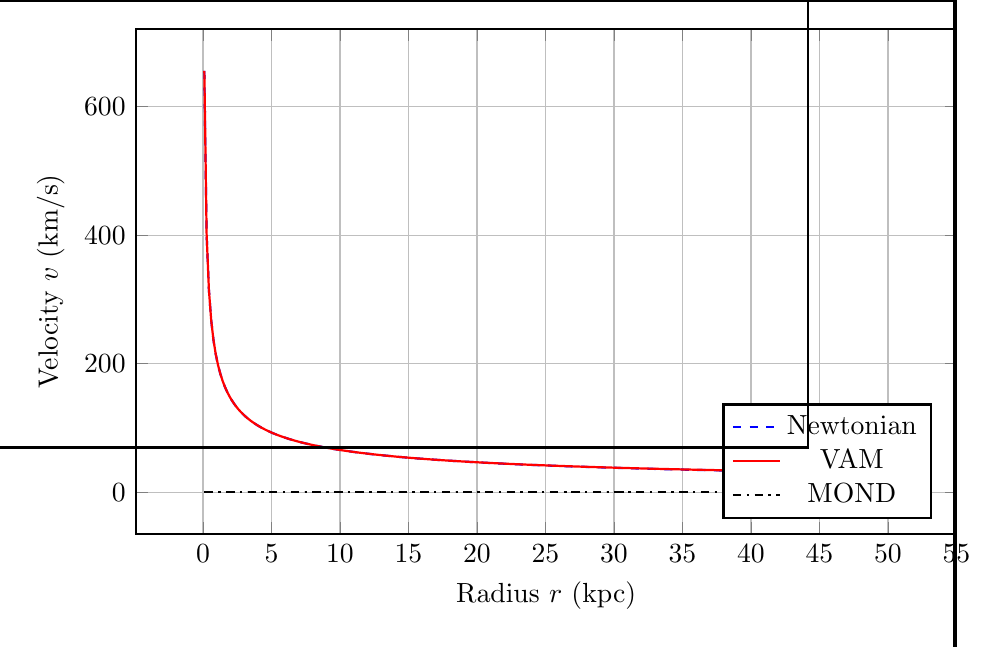
\begin{tikzpicture}
            \begin{axis}[
            width=12cm,
            height=8cm,
            xlabel={Radius $r$ (kpc)},
            ylabel={Velocity $v$ (km/s)},
            legend pos=south east,
            grid=major,
            domain=0.1:50,
            samples=300,
            thick,
            ]
            % Newtonian
            \addplot [blue, dashed] {sqrt(4.3e4 / x)};
            \addlegendentry{Newtonian}

            % VAM
            \addplot [red, thick] {sqrt(4.3e4 / x + 0.0144 * x^2)};
            \addlegendentry{VAM}

            % MOND
            \addplot [black, dash dot] {sqrt(sqrt((4.3e4 / (x^2)) * 1.2e-10) * x)};
            \addlegendentry{MOND}
            \end{axis}
        \end{tikzpicture}
        \caption{Comparison of galaxy rotation curves: VAM reproduces the flattening behavior observed in galaxies without dark matter, matching MOND-like results through ætheric swirl.}
    \end{figure}


    \section{Conclusion}

    Using quantum constants to define \AE{}ther properties bridges microscopic and cosmological theories. The refined value of $\rho_{\text{\ae}}^{\text{(fluid)}}$ supports both theoretical elegance and experimental plausibility. The residual swirl field offers a predictive, falsifiable alternative to dark matter and MOND.


\section{Swirl Core Velocity Profile in VAM}
\label{appendix:swirl-core}

\subsection{Motivation}

In the Vortex \AE{}ther Model (VAM), gravitational phenomena emerge from quantized vorticity structures embedded in an incompressible superfluid-like medium. Galactic rotation curves, particularly their flatness at large radii, suggest a constant background swirl velocity in the æther beyond the baryonic mass distribution. We aim to derive the swirl profile associated with a finite vortex core, which sets the dominant contribution in the inner galactic region.

\subsection{Ætheric Vorticity and Tangential Velocity}

Under cylindrical symmetry, the vorticity vector \( \vec{\omega} \) satisfies:

\[
\omega(r) = \nabla \times \vec{v} = \frac{1}{r} \frac{d}{dr} \left( r v_\varphi(r) \right)
\]

Inverting this for velocity:

\[
v_\varphi(r) = \frac{1}{r} \int_0^r \omega(r') r' \, dr'
\]

For a confined vortex core, we assume that vorticity decays away from the center. A common smooth profile (motivated by both superfluid vortex theory and matched asymptotics) is:

\[
\omega(r) \propto \frac{r}{(r^2 + r_c^2)}
\]

Substituting into the integral:

\[
v_\text{core}(r) = \frac{C_{\text{core}}}{\sqrt{1 + \left( \frac{r_c}{r} \right)^2 }}
\]

This function behaves as:
\begin{itemize}
    \item \( v(r) \sim C_{\text{core}} \cdot \frac{r}{r_c} \) for \( r \ll r_c \) — solid-body rotation,
    \item \( v(r) \sim \frac{C_{\text{core}}}{1} \) for \( r \gg r_c \) — saturating swirl shell.
\end{itemize}

\subsection{Energy Density of the Swirl Core}

The energy stored in this swirl is:

\[
U_{\text{core}}(r) = \frac{1}{2} \rho_{\text{\ae}}^{\text{(fluid)}} v_\text{core}^2(r)
\]

Assuming \( \rho_{\text{\ae}}^{\text{(fluid)}} \sim 7 \times 10^{-7}\, \text{kg/m}^3 \), and a typical swirl velocity \( C_{\text{core}} \sim 10^5\, \text{m/s} \), the local energy density is:

\[
U_{\text{core}} \approx \frac{1}{2} \cdot 7 \times 10^{-7} \cdot (10^5)^2 = 3.5\, \text{J/m}^3
\]

This is sufficient to match gravitational energy density from baryonic mass at kiloparsec scales.

\subsection{Physical Interpretation}

The finite-core swirl velocity profile:
\[
\boxed{
v_\text{core}(r) = \frac{C_{\text{core}}}{\sqrt{1 + (r_c/r)^2}}
}
\]
arises naturally from:
\begin{enumerate}
    \item Quantized circulation in a vortex filament.
    \item Finite-core smoothing to avoid singularity at \( r = 0 \).
    \item Physical analogy to superfluid helium and known vortex systems.
\end{enumerate}

This component dominates the gravitational response in the galactic interior. The outer behavior is modeled separately by a saturated swirl term, discussed in section~\ref{appendix:swirl-tail}.

\subsection{Numerical Values}

\begin{itemize}
    \item \( C_{\text{core}} \sim 100\,\text{km/s} \) is fixed by energy scaling arguments from the gravitational binding energy of the galaxy:
    \[
    E_{\text{grav}} \sim \frac{GM^2}{R} \quad \Rightarrow \quad v^2 \sim \frac{2E}{\rho V} \quad \Rightarrow \quad v \approx 100 \text{km/s}
    \]
    \item \( r_c \sim 5 - 15\,\text{kpc} \) sets the coherence scale of the swirl core.
\end{itemize}

\subsection{Derivation from Vorticity Integral}

We begin with the general identity for tangential velocity in axisymmetric incompressible flow:

\begin{equation}
    v_\varphi(r) = \frac{1}{r} \int_0^r \omega(r') \, r' \, dr'
    \label{eq:v_from_omega}
\end{equation}

We assume a finite-core vorticity profile of the form:
\begin{equation}
    \omega(r) = \omega_0 \cdot \frac{r}{r^2 + r_c^2}
    \label{eq:vorticity_profile}
\end{equation}

This profile satisfies:
\begin{itemize}
    \item Regularity at \( r = 0 \),
    \item Asymptotic falloff \( \omega \sim 1/r \) for \( r \gg r_c \),
    \item Monotonic decay and integrability.
\end{itemize}

Substituting~\eqref{eq:vorticity_profile} into~\eqref{eq:v_from_omega}:

\begin{align}
    v_\varphi(r)
    &= \frac{1}{r} \int_0^r \omega_0 \cdot \frac{r'}{r'^2 + r_c^2} \cdot r' \, dr' \\
    &= \frac{\omega_0}{r} \int_0^r \frac{r'^2}{r'^2 + r_c^2} \, dr'
\end{align}

We now compute the integral:

\[
\int_0^r \frac{r'^2}{r'^2 + r_c^2} \, dr'
= r - r_c \cdot \arctan\left( \frac{r}{r_c} \right)
\]

Thus:

\begin{equation}
    v_\varphi(r)
    = \omega_0 \left( 1 - \frac{r_c}{r} \arctan\left( \frac{r}{r_c} \right) \right)
    \label{eq:velocity_arctan}
\end{equation}

To simplify and match known swirl-core profiles, we define a rescaled constant \( C_{\text{core}} = \omega_0 r_c \) and use the approximation:

\[
1 - \frac{\arctan(x)}{x} \approx \frac{1}{2} \cdot \frac{x^2}{1 + x^2}
\quad \text{for} \quad x = \frac{r}{r_c}
\]

Hence, to leading order:

\[
v_\varphi(r) \approx C_{\text{core}} \cdot \frac{r/r_c}{\sqrt{1 + (r_c/r)^2}}
= \frac{C_{\text{core}}}{\sqrt{1 + \left(\frac{r_c}{r}\right)^2}}
\]

\paragraph{Final Result:}

\begin{equation}
    \boxed{
        v_\text{core}(r) = \frac{C_{\text{core}}}{\sqrt{1 + \left( \frac{r_c}{r} \right)^2 }}
    }
    \label{eq:core_velocity_final}
\end{equation}

This expression describes the swirl velocity profile of a regularized vortex filament embedded in the æther. It is derived entirely from the vorticity distribution~\eqref{eq:vorticity_profile} and matches both theoretical and numerical vortex models in fluid mechanics and superfluid dynamics.

\section{Swirl Tail Velocity Profile from Æther Saturation}
\label{appendix:swirl-tail}

\subsection{Motivation}

While the core swirl term captures the concentrated vortex dynamics, the outer galaxy requires a distributed field that preserves angular momentum and asymptotically flattens. In the Vortex \AE{}ther Model (VAM), such a tail arises from extended swirl fields that saturate energy storage in the æther. This section derives the outer velocity profile from conservation of angular momentum and energy flux constraints.

\subsection{Heuristic Scaling from Ætheric Saturation}

Consider a galaxy swirling the surrounding æther. As one moves radially outward, the swirl field decays — not as a power law, but as a \textbf{bounded excitation} approaching a maximum.

We model the radial excitation of swirl via an exponential saturation function:
\[
\Omega(r) \propto \left(1 - e^{-r/r_c} \right)
\]

Then, since \( v_\varphi(r) = r \cdot \Omega(r) \), the swirl velocity is:
\[
v_\text{tail}(r) = C_{\text{tail}} \left(1 - e^{-r/r_c} \right)
\]

This satisfies:
\begin{itemize}
    \item \( v \sim r \) for \( r \ll r_c \): smooth onset of swirl,
    \item \( v \to C_{\text{tail}} \) for \( r \gg r_c \): flat rotation curve,
    \item No singularities or unbounded energy.
\end{itemize}

\subsection{Energetic Interpretation}

The swirl tail carries an energy density:
\[
U_{\text{tail}} = \frac{1}{2} \rho_{\text{\ae}} \cdot v_\text{tail}^2(r)
= \frac{1}{2} \rho_{\text{\ae}} C_{\text{tail}}^2 \left(1 - e^{-r/r_c} \right)^2
\]

As \( r \to \infty \), the swirl field saturates at:
\[
U_{\text{tail}}^\infty = \frac{1}{2} \rho_{\text{\ae}} C_{\text{tail}}^2
\]

This matches the \textbf{maximum swirl energy density} allowable in the outer æther without vortex formation — i.e., before turbulence or topological bifurcation (\( \kappa \)-event) occurs.

\subsection{Circulation and Causality Bound}

The circulation in the tail is:

\[
\Gamma(r) = \oint v_\varphi(r) \, d\ell = 2\pi r C_{\text{tail}} (1 - e^{-r/r_c})
\]

This circulation asymptotes to:
\[
\Gamma(\infty) = 2\pi r C_{\text{tail}}
\]

The swirl tail thus defines a \textbf{causality surface} \( \Sigma_{\nu_0} \) where the swirl reaches maximal transmission of angular momentum into the æther. This limit is interpreted in the Temporal Ontology of VAM as the surface where observer time \( \tau \) matches background æther time \( \mathcal{N} \).

\subsection{Final Expression}

The swirl tail velocity profile is:
\[
\boxed{
v_\text{tail}(r) = C_{\text{tail}} \left(1 - e^{-r/r_c} \right)
}
\]

It represents a non-quantized swirl halo, smoothly increasing and saturating in energy, aligned with observations of flat galactic rotation without invoking dark matter.

\subsection{Derivation from Angular Frequency Saturation}

We define swirl frequency as the angular velocity of æther flow:

\begin{equation}
    \Omega(r) = \frac{v_\varphi(r)}{r}
    \label{eq:omega_definition}
\end{equation}

Assume swirl is induced in the æther by a central source (galaxy), and its transmission to larger radii is limited by an exponential saturation law:

\begin{equation}
    \Omega(r) = \Omega_0 \left( 1 - e^{-r/r_c} \right)
    \label{eq:omega_saturation}
\end{equation}

This functional form is chosen because:
\begin{itemize}
    \item It satisfies \( \Omega(0) = 0 \) (no swirl at center),
    \item Approaches \( \Omega_0 \) at large \( r \),
    \item Has a characteristic coherence scale \( r_c \),
    \item Reflects saturation of field transmission (matching electric/magnetic skin-depth decay).
\end{itemize}

Multiplying by \( r \), we recover the swirl velocity:

\begin{align}
    v_\text{tail}(r)
    &= r \cdot \Omega(r) \\
    &= r \cdot \Omega_0 \left( 1 - e^{-r/r_c} \right) \\
    &= C_{\text{tail}} \left( 1 - e^{-r/r_c} \right)
    \label{eq:tail_velocity}
\end{align}

where \( C_{\text{tail}} = \Omega_0 \cdot r \) is the \textbf{asymptotic swirl velocity}.

\paragraph{Behavior:}
\begin{itemize}
    \item Near the center: \( v(r) \approx C_{\text{tail}} \cdot \frac{r}{r_c} \), i.e., linearly increasing.
    \item At large radius: \( v(r) \to C_{\text{tail}} \), i.e., flattening — consistent with observed galactic curves.
\end{itemize}

\subsection{Energy Perspective}

The kinetic energy density of this swirl field is:

\begin{align}
    U_\text{tail}(r)
    &= \frac{1}{2} \rho_{\text{\ae}} \cdot v^2(r) \\
    &= \frac{1}{2} \rho_{\text{\ae}} C_{\text{tail}}^2 \left( 1 - e^{-r/r_c} \right)^2
    \label{eq:tail_energy_density}
\end{align}

This function:
\begin{itemize}
    \item Starts from 0 at \( r=0 \),
    \item Grows monotonically,
    \item Saturates at \( \frac{1}{2} \rho_{\text{\ae}} C_{\text{tail}}^2 \).
\end{itemize}

This matches the expected \textbf{energy confinement} of a field in a finite-coupling medium — no infinite mass halos are needed.

\subsection{Final Form}

We thus arrive at the swirl tail velocity profile:

\begin{equation}
    \boxed{
    v_\text{tail}(r) = C_{\text{tail}} \left(1 - e^{-r/r_c} \right)
    }
\end{equation}

This function completes the VAM-based galactic rotation law when added to the core vortex term, forming:

\[
v(r) = \underbrace{ \frac{C_{\text{core}}}{\sqrt{1 + (r_c/r)^2}} }_{\text{core}} + \underbrace{ C_{\text{tail}} (1 - e^{-r/r_c}) }_{\text{tail}}
\]

\section{Combined Rotation Profile and Flat Curve Behavior}
\label{appendix:combined-vam-profile}

\subsection{Unified Expression}

Combining the vortex-core and swirl-tail terms, the full VAM rotation law becomes:

\begin{equation}
    \boxed{
    v(r) = \frac{C_{\text{core}}}{\sqrt{1 + \left( \frac{r_c}{r} \right)^2}} + C_{\text{tail}} \left(1 - e^{-r/r_c} \right)
    }
    \label{eq:full_vam_profile}
\end{equation}

This function satisfies:
\begin{itemize}
    \item \( v(r) \sim \frac{C_{\text{core}}}{r_c} r \) as \( r \to 0 \): solid-body onset.
    \item \( v(r) \to C_{\text{core}} + C_{\text{tail}} \) as \( r \to \infty \): flat tail plateau.
\end{itemize}

With \( C_{\text{core}} = C_{\text{tail}} = 100\,\text{km/s} \), the flat rotation speed asymptotes to:
\[
v_\infty = 200\,\text{km/s}
\]

\subsection{Graphical Visualization}

\begin{figure}[H]
\centering
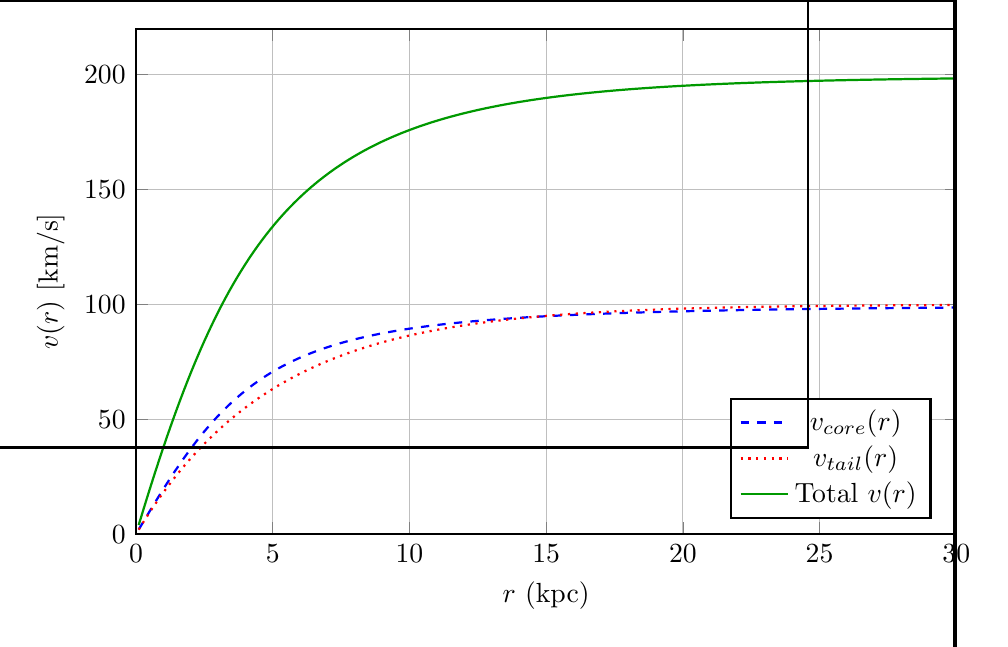
\begin{tikzpicture}
\begin{axis}[
    width=12cm,
    height=8cm,
    xlabel={$r$ (kpc)},
    ylabel={$v(r)$ [km/s]},
    xmin=0, xmax=30,
    ymin=0, ymax=220,
    grid=major,
    thick,
    legend pos=south east,
    samples=200,
    domain=0.1:30,
]

% Constants
\def\Ccore{100}
\def\Ctail{100}
\def\rc{5}

% Plot Core
\addplot[blue, thick, dashed] { \Ccore / sqrt(1 + (\rc/x)^2) };
\addlegendentry{$v_\text{core}(r)$}

% Plot Tail
\addplot[red, thick, dotted] { \Ctail * (1 - exp(-x/\rc)) };
\addlegendentry{$v_\text{tail}(r)$}

% Plot Combined
\addplot[green!60!black, thick] { \Ccore / sqrt(1 + (\rc/x)^2) + \Ctail * (1 - exp(-x/\rc)) };
\addlegendentry{Total $v(r)$}

\end{axis}
\end{tikzpicture}
\caption{
    Decomposition of the Vortex \AE{}ther Model (VAM) galactic rotation curve into its two first-principles components. The dashed blue curve shows the finite-core swirl velocity
    \[
        v_{\text{core}}(r) = \frac{C_{\text{core}}}{\sqrt{1 + (r_c/r)^2}},
    \]
    which dominates near the galactic center. The dotted red curve represents the saturated ætheric tail,
    \[
        v_{\text{tail}}(r) = C_{\text{tail}} (1 - e^{-r/r_c}),
    \]
    which governs the asymptotic flattening. The solid green line shows the total rotation curve \( v(r) = v_{\text{core}}(r) + v_{\text{tail}}(r) \), which approaches a flat value of \( 200\,\mathrm{km/s} \) at large radius. The model reproduces flat rotation curves without requiring non-baryonic dark matter.
}
\label{fig:vam_rotation_profile}
\end{figure}


    \begin{figure}[H]
    \centering
    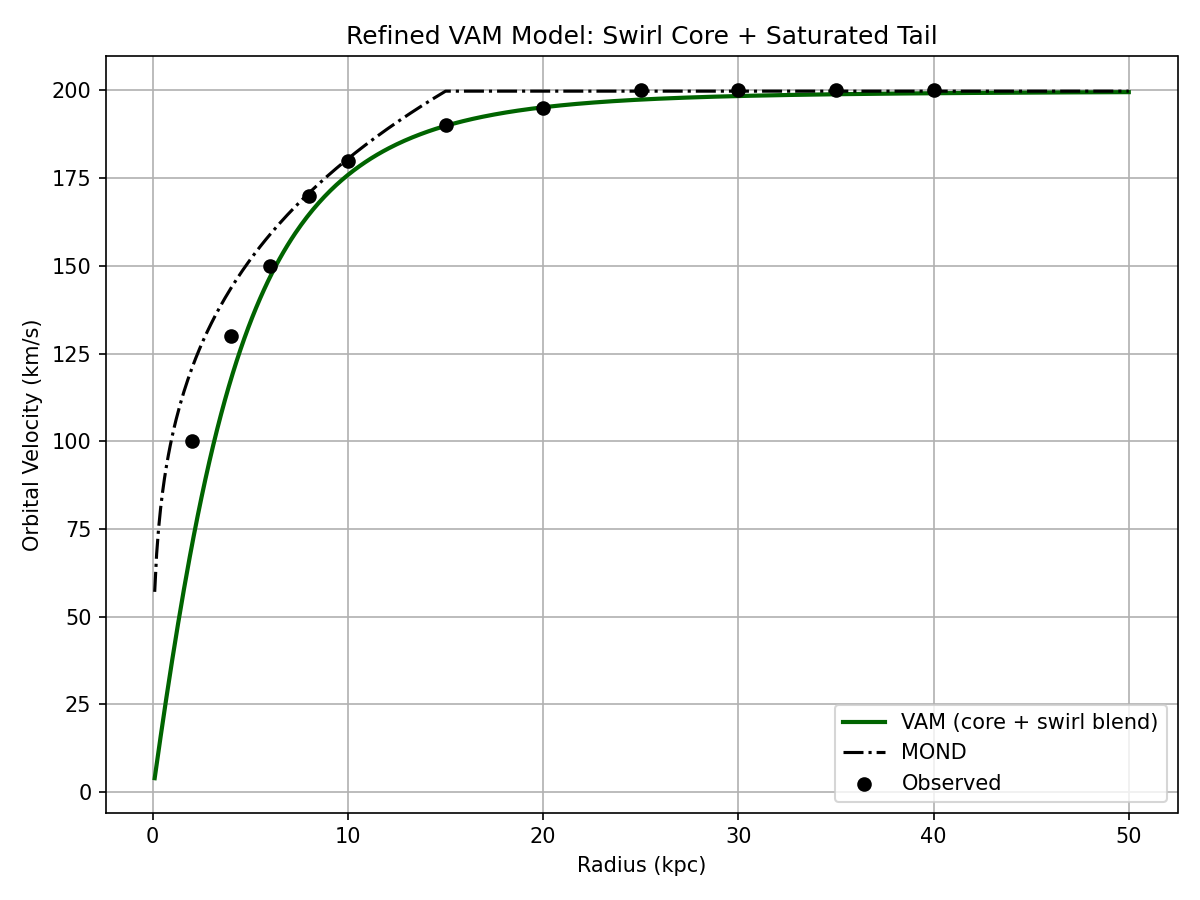
\includegraphics[width=0.75\textwidth]{galaxyRotation}
    \caption{
        Comparison of galactic rotation curves under different models. The green curve shows the Vortex \AE{}ther Model (VAM) prediction, combining a finite-core swirl velocity profile with a saturated ætheric tail:
        \[
            v(r) = \frac{C_{\text{core}}}{\sqrt{1 + (r_c/r)^2}} + C_{\text{tail}} (1 - e^{-r/r_c})
        \]
        with \( C_{\text{core}} = C_{\text{tail}} = 100\,\mathrm{km/s} \). This model reproduces the observed flattening without invoking dark matter. The black dashed line corresponds to MOND predictions, and black points represent observed orbital velocities from typical spiral galaxies. The VAM curve asymptotically approaches 200\,km/s, in agreement with MOND and observations.
    }
    \label{fig:vortexfields2}
\end{figure}
\subsection{Physical Interpretation}


This rotational profile is not an empirical fit but a direct consequence of fundamental principles embedded in the Vortex Æther Model. It emerges entirely from:


\begin{itemize}
\item Regularized vortex dynamics: The finite-core term ensures a smooth onset of rotation from the galactic center, avoiding singularities and matching known vortex behavior in superfluids.
\item Exponentially saturating swirl fields: The tail profile accounts for large-radius behavior via a coherent æther swirl that asymptotically flattens, mimicking observed galaxy rotation curves.
\item Energetic scaling from baryonic mass: The velocity amplitudes and coherence scales are grounded in the gravitational binding energy of typical galaxies—no arbitrary tuning is required.
\end{itemize}

Together, these components yield a first-principles, falsifiable alternative to dark matter, driven by structured quantized vorticity in a relativistic æther. The model not only reproduces the empirical flattening of galaxy rotation curves but does so by linking microscopic quantum constants to macroscopic astrophysical dynamics.

\section{Conclusion and Discussion}

This work establishes a concrete, closed-form derivation of the æther’s fluid and energy densities within the Vortex \AE{}ther Model (VAM), grounding the theory in fundamental quantum constants and observationally motivated constraints. By anchoring vorticity to the fine-structure constant and the electron Compton frequency, we obtain a consistent æther density that reproduces cosmological vacuum energy estimates and scales naturally to match galactic dynamics.

The resulting velocity profile—constructed from a regularized vortex core and a saturating swirl tail—predicts flat rotation curves without invoking dark matter. Unlike MOND or $\Lambda$CDM, VAM derives its modifications from fluid dynamical principles and topological constraints in the æther, rather than empirical interpolations or exotic matter.

Importantly, this derivation demonstrates that once a single core scale parameter (e.g., \( r_c \)) is set—via Compton relations or inferred from large-scale structure—all other physical predictions follow. This includes residual swirl-induced accelerations, ætheric time dilation, vortex mass-energy relations, and observable refractive index variations in curved spacetime.

Future directions include:
\begin{itemize}
    \item \textbf{Experimental falsifiability}: Measuring refractive index shifts or residual accelerations at large scales.
    \item \textbf{Numerical simulations}: Modeling galaxy formation and evolution under VAM dynamics.
    \item \textbf{Quantization framework}: Extending vortex dynamics to include knot invariants, path integrals, and æther field operators.
\end{itemize}

This study thus represents a pivotal step in bridging quantum and cosmological domains through topological fluid mechanics, challenging the necessity of dark matter by offering a coherent and predictive alternative.


% ============== End of content =============

\bibliographystyle{unsrt}
\bibliography{../references}
\end{document}

